%%\documentclass[aspectratio=1610]{beamer}
\documentclass[xcolor=table,xcolor=dvipsnames]{beamer}
%
%%%%%%%%%%%%%%%%%%%%%%%%%%%%%%%%%%%%
%% Common preamble
%%%%%%%%%%%%%%%%%%%%%%%%%%%%%%%%%%%%
% PAGE
%% \usepackage{fullpage}
% FONTS
\usepackage{lmodern} % enhanced version of computer modern
\usepackage[T1]{fontenc} % for hyphenated characters
\usepackage{amssymb}
\usepackage{mathtools} % contains amsmath which comes with align
\usepackage{amsthm}
\usepackage{microtype} % some compression
%%%%%%%%%%%%%%%%%%%%%%%%%%%%%%%%%%%%
\usepackage{tikz}
\usepackage{multirow}
\usetikzlibrary{spy,shadows,arrows,shapes,positioning,calc,backgrounds,fit,automata}


\newcommand{\completed}{\tikz{\draw[fill=green,opacity=1,line width=1pt] circle(1ex);}}
\newcommand{\ongoing}{\tikz{\draw[fill=yellow,opacity=1,line width=1pt] circle(1ex);}}
\newcommand{\notstarted}{\tikz{\draw[fill=red,opacity=1,line width=1pt] circle(1ex);}}

\newcommand{\newcompleted}{\tikz{\draw[fill=green,opacity=1,line width=1pt]
(-.2,-.2) rectangle (.15,.15);}}
\newcommand{\newongoing}{\tikz{\draw[fill=yellow,opacity=1,line width=1pt]
(-.2,-.2) rectangle (.15,.15);}}
\newcommand{\newnotstarted}{\tikz{\draw[fill=red,opacity=1,line width=1pt]
(-.2,-.2) rectangle (.15,.15);}}

\newcommand{\rowcon}[2]{\cellcolor{#2}\parbox{2cm}{\small #1}}

\newcommand{\dunder}[1]{\underline{\underline{#1}}}
\newcommand{\calc}{\mathcal{C}}
\newcommand{\cali}{\mathcal{I}}
\newcommand{\calb}{\mathcal{B}}
\newcommand{\calo}{\mathcal{O}}
\newcommand{\cals}{\mathcal{S}}
\newcommand{\calp}{\mathcal{P}}
\newcommand{\domb}{\mathbb{B}}
\newcommand{\dmax}{d_{\max}}
\newcommand{\cost}{\text{cost}}
\newcommand{\comment}[1]{{\color{red}#1}}
\newcommand{\wmin}{w_{\min}}
\newcommand{\copt}{C_{\text{OPT}}}
\newcommand{\TikZ}{Ti\textit{k}Z\xspace}
\newcommand{\tuta}{\emph{T. absoluta}}
\newcommand{\prempt}{\textsc{PREMpT}}
\definecolor{col1}{HTML}{D53E4F}
\definecolor{col2}{HTML}{F46D43}
\definecolor{col3}{HTML}{FDAE61}
\definecolor{col4}{HTML}{FEE08B}
\definecolor{col5}{HTML}{E6F598}
\definecolor{col6}{HTML}{ABDDA4}
\definecolor{col7}{HTML}{66C2A5}
\definecolor{col8}{HTML}{3288BD}


%%
\title[]{Assessment of Invasive Alien Plant Species Distribution in the Chitwan Annapurna Landscape (CHAL) region ,Nepal with the Application of satellite Imagery}
\date[Sep 24, 2019]{Sep 24, 2019}
\author[A.~Adiga]{Abhijin Adiga and Madhav Marathe (PI)}
\institute[]{
    \mbox{}\hspace{.9cm}\raisebox{.6cm}{
\includegraphics[width=4cm]{figs/uva_horiz_rgb.png}}\hspace{.9cm}\raisebox{.2cm}{
\includegraphics[width=2.5cm]{figs/bivt_logo.pdf}}\\
\raisebox{.55cm}{
\includegraphics[width=3.4cm]{figs/IPM-Innovation-Lab-header-logo.png}}~\hspace{.2cm}\raisebox{.4cm}{
\includegraphics[width=3.4cm]{figs/FtF.pdf}}~\hspace{.2cm}\raisebox{.4cm}{
\includegraphics[width=3.1cm]{figs/usaid.pdf}}
}
%% ----------------------------------------------------------------------
%%
\usetheme{CambridgeUS}
\useoutertheme{nssac}

%% This ``scales'' the font. Don't extend too much beyond 128x96
%% Uncomment the next line for default sizes:
\geometry{paperwidth=140mm,paperheight=105mm}
\setbeamercolor{block title}{use=structure,fg=white,bg=black!75!white}
\setbeamercolor{block body}{use=structure,fg=black,bg=black!10!white}
\beamertemplatenavigationsymbolsempty

\begin{document}
%% ----------------------------------------------------------------------

\begin{frame}
\titlepage
\end{frame}
%%
%% ----------------------------------------------------------------------
%%
\begin{frame}
\frametitle{Main objectives}
\setbeamercovered{invisible}%{dynamic}
\begin{enumerate}
    \item Develop a deep learning based framework to create species
    distribution maps. \newongoing
    \item Apply this framework along with network (agent-based) models to
    study the spatio-temporal spread of the focus invasive species.
    \newnotstarted
\end{enumerate}
Team: 1 postdoc (Institute funds) + two interns (summer/full year) + two
research scientists
\end{frame}
%%
%% ---------------------------------------------------------------------- 
%%
\begin{frame}
\frametitle{Deep learning approach} 
\centering
\begin{tikzpicture}
    \node {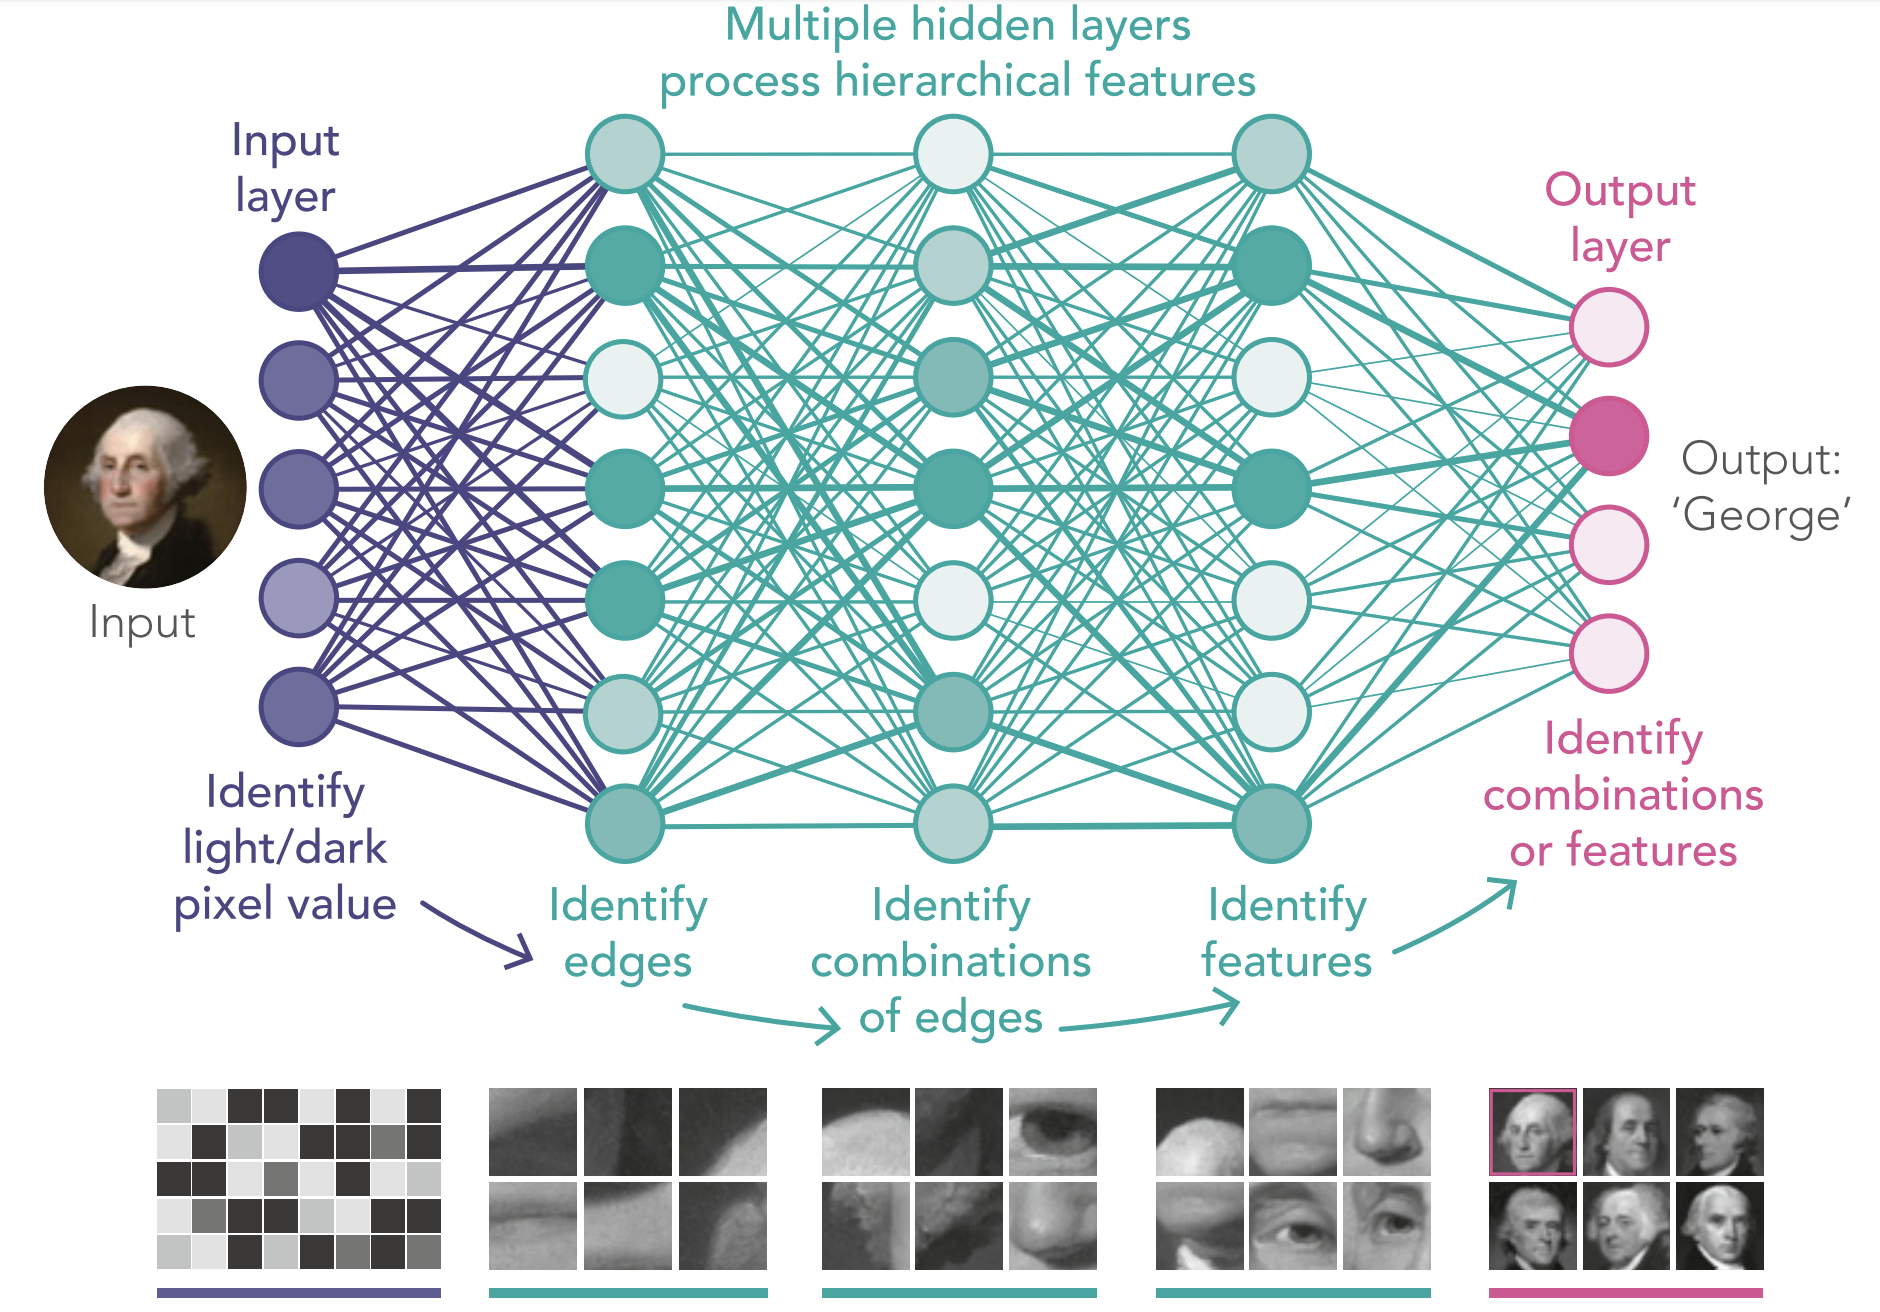
\includegraphics[width=.8\textwidth]{figs/deep_learning.png}};
    \node at (-4.9,.9) {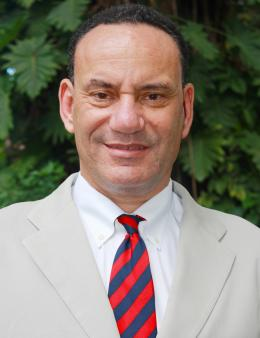
\includegraphics[width=2cm]{figs/john.jpg}};
    \node[fill=white,text width=1.3cm,align=center] at (4.8,1) {Output 'John'};
    \node[anchor=west] at (-4.3,-4) {\small Courtesy: M. Waldrop, PNAS};
\end{tikzpicture}
\end{frame}
%%
%% ---------------------------------------------------------------------- 
%%
\begin{frame}
\frametitle{Deep learning approach} 
\begin{itemize}
    \item Diverse applications, superior performance (particularly, image
    related), (almost) zero interpretability.
    \item Has been around since 1970s.
    \item Enabled by clever algorithms and HPC, it got a boost in the early
    2000s.
    \item Enabled by availability of large amounts of data.
    \item Promise: Hardly any work on applying it to invasive species mapping.
\end{itemize}
\end{frame}
%%
%% ---------------------------------------------------------------------- 
%%
\begin{frame}
\frametitle{Challenges} 
\begin{itemize}
    \item Data inadequacy
    \begin{itemize}
    \item Difficulties with field survey.
    \item High-resolution imagery is expensive.
    \item Sparse coverage (unlike cropland detection).
    \item Moderate-resolution (Landsat) might not be adequate.
    \end{itemize}
    \item Methods
    \begin{itemize}
        \item Very little previous work
        \item Class imbalance
    \end{itemize}
\end{itemize}
\end{frame}
%%
%% ---------------------------------------------------------------------- 
%%
\begin{frame}
\frametitle{Our framework} 
{
\centering
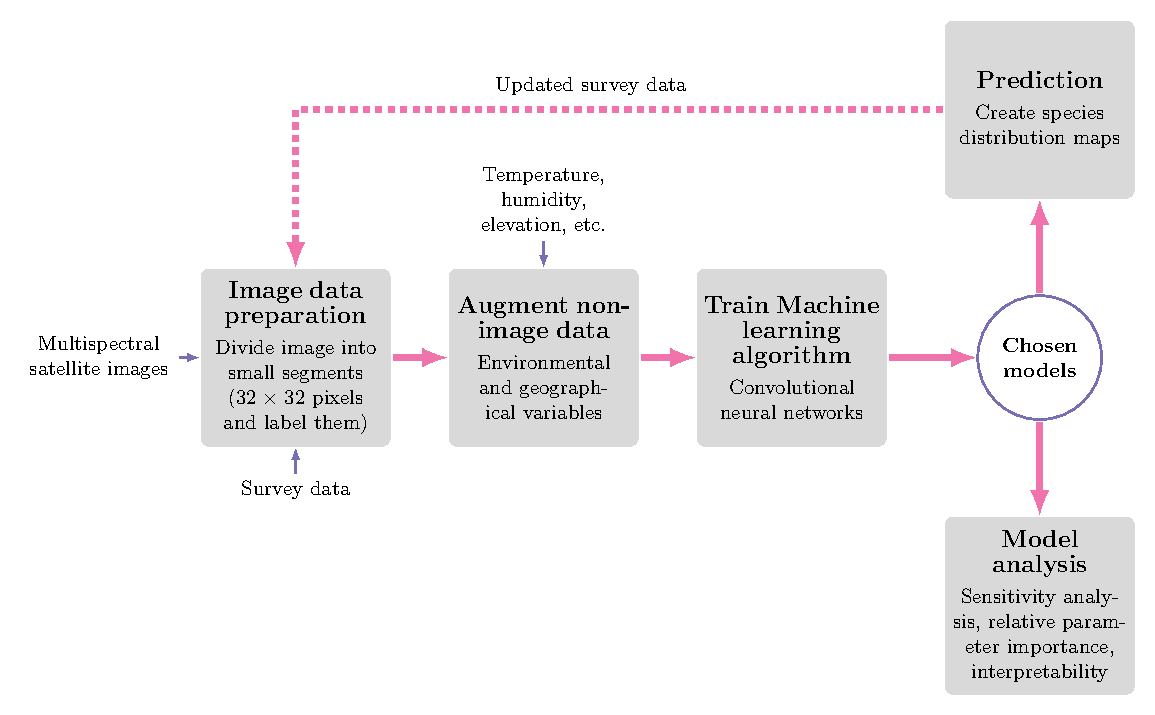
\includegraphics[width=.99\textwidth]{figs/pipeline.pdf}
}
\end{frame}
%%
%% ---------------------------------------------------------------------- 
%%
\begin{frame}
\frametitle{Data and experiments} 
\begin{itemize}
    \item Survey was conducted in two phases: Phase I and Phase~II.
    \item Experimented with multiple CNN architectures and chose the model with the best accuracy.
    \begin{itemize}
\item Training accuracy – how well the model learns the training data.
\item Validation accuracy – how well the model generalizes to unseen data.
\end{itemize}
\item Phase I data: 61, 32x32, 8 band digital globe images of location where lantana is present/absent (field expert annotated).
\item For model parameter learning, insufficient and imbalanced data.
\item Phase II data: 225 images
\end{itemize}
\end{frame}
%%
%% ---------------------------------------------------------------------- 
%%
\begin{frame}
    \frametitle{Results}
\begin{itemize}
    \item Trained on Phase I data, tested on unseen Phase~II data:
    \begin{itemize}
        \item Best model: 76\% accuracy
        \item Average model: 64\% accuracy
    \end{itemize}
    \item Trained on Phase~II data.
    \begin{itemize}
        \item Slight improvement in accuracy.
    \end{itemize}
\end{itemize}
Manuscript under preparation on {Lantana} distribution.
\end{frame}
%%
%% ---------------------------------------------------------------------- 
%%
\begin{frame}
\frametitle{Ongoing work} 
Two main thrusts
\begin{itemize}
    \item Understanding spatiotemporal spread.
    \begin{itemize}
        \item Incorporating high-resolution images: New (2019, 2018) and
        old (2011, 2012)
        \item Incorporating moderate-resolution images (Landsat): 10 and 20
        year old images.
        \item Pending: using network models (like in \tuta)
    \end{itemize}
    \item Augmenting satellite imagery with Environmental/geographic
    variables: temperature, humidity, altitude, elevation, etc.
    \begin{itemize}
        \item Interpretability
    \end{itemize}
\end{itemize}
\end{frame}
%%
%% ---------------------------------------------------------------------- 
%%
\end{document}
